% 2005 年全国卷Ⅰ理科第 8 题：二次函数的四个图象选项
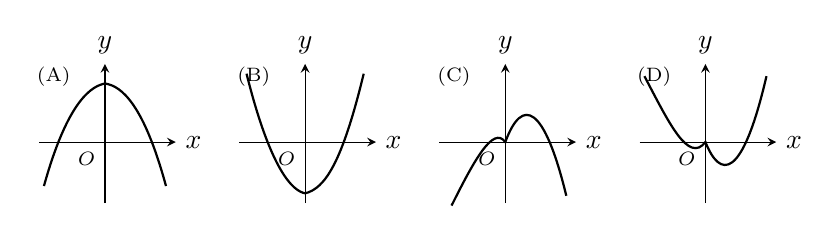
\begin{tikzpicture}[>=stealth,scale=0.62]
  \foreach \dx/\lab in {0/{(A)},4.1/{(B)},8.2/{(C)},12.3/{(D)}} {
    \begin{scope}[xshift=\dx cm]
      \draw[->] (-1.35,0)--(1.45,0) node[right] {$x$};
      \draw[->] (0,-1.25)--(0,1.6) node[above] {$y$};
      \node[font=\scriptsize] at (-1.05,1.35) {\lab};
      \node[below left,font=\scriptsize] at (0,0) {$O$};
    \end{scope}
  }
  % A: downward, positive intercept.
  \begin{scope}
    \draw[thick] (-1.25,-0.9)..controls(-0.75,0.9) and (-0.25,1.15)..(0,1.2)
      ..controls(0.35,1.15) and (0.8,0.75)..(1.25,-0.9);
  \end{scope}
  % B: upward, negative intercept, roots near -1 and 1.
  \begin{scope}[xshift=4.1cm]
    \draw[thick] (-1.2,1.4)..controls(-0.7,-0.6) and (-0.25,-1.0)..(0,-1.05)
      ..controls(0.4,-0.95) and (0.75,-0.45)..(1.2,1.4);
  \end{scope}
  % C: downward through the origin.
  \begin{scope}[xshift=8.2cm]
    \draw[thick] (-1.1,-1.3)..controls(-0.65,-0.4) and (-0.25,0.35)..(0,0)
      ..controls(0.35,0.95) and (0.8,0.75)..(1.25,-1.1);
  \end{scope}
  % D: upward through the origin with negative initial slope.
  \begin{scope}[xshift=12.3cm]
    \draw[thick] (-1.25,1.35)..controls(-0.75,0.4) and (-0.35,-0.45)..(0,0)
      ..controls(0.3,-0.75) and (0.75,-0.8)..(1.25,1.35);
  \end{scope}
\end{tikzpicture}
